\documentclass[a4paper,12pt]{article}
\parindent 0pt
\parskip 1mm
\usepackage[dvips]{epsfig}

\begin{document}

\begin{center}
{\Large\bf CN 510 - Principles and Methods of Cognitive and Neural Modeling}

\bigskip

{\large\bf Assignment \# 2}
\smallskip

{\large\bf John Joseph}
\end{center}

\bigskip
{\bf Part 1 : Handmade Euler Numerical Integration}
{\bf Introduction}
\bigskip

Part 1 of this assignment asks us to numerically simulate the Leaky Integrator model of the neuron using the Euler Method. I must come clean, here - in the previous assignment I included an Euler simulation, as well as another simulation using the Runge-Kutta 4 method, with the intent of impressing the instructor. I had no idea we'd be doing it for this assignment, but as a result I am relying on data generated from Assignment 1. 

\vspace{2mm}

I chose to use the results of the RK4 simulation in this report, since I've been lead to believe they are more accurate. To the grader - if you were expecting Euler and would like to see those results, please let me know. It's no trouble to send a revised version of this report using the Euler method, and I understand that it may be a bother to determine if my results are indeed correct. 

\vspace{2mm}

That being said, I ran the simulation using RK4 and a time step of $\Delta t=0.05$ seconds. The Euler Integration method works by advancing the current state of our variable using its calculated rate of change and an arbitrarily low time step. The RK4 method works by calculating the rate of change at several key points about this time step, generating a weighted average of those rates, and then advancing the current value using the averaged rate as one would in an Euler simulation. This requires more computation, but for an assignment like this it's all pretty negligible. 

\vspace{2mm}

The simulation was run twice for ten seconds each using two different decay rates (labeled as $A$). For each simulation, an input current $I$ was supplied for the first five seconds. As discussed in the previous report, the results of the RK4 solution were at all times equal to those of the Analytic and Rotter-Deissmann solution. 

\vfil\eject

{\bf Results}
\bigskip

The results of the numerical simulations are the same as they were in the previous assignment, but the context of this assignment merits a bit of discussion. Given that this assignment demands we turn our input current on and off during single simulation, we must be aware of the importance of rates of convergence and how the method of simulation can determine the final outcome. 

\vspace{2mm}

The table below shows how the Leaky Integrator behaves as it approaches equilibrium. As derived in the previous assignment, the Leaky Integrator model converges to $\frac{I}{A}$, the quotient of its two parameters. 

\vspace{4mm}

\begin{tabular}{ | l | l | l | l | l | l | l |}
  \hline
    Time(seconds) & A & I & I/A & Euler & Analytic & Difference \\ \hline
    5 & 1 & 5 & 5 & 4.970397 & 4.966310 & 0.004087 \\ \hline
    10 & 1 & 0 & 0 & 0.027972 & 0.031841 & 0.003869 \\ \hline
    5 & 2 & 5 & 2.5 & 2.499934 & 2.499888 & 0.000046 \\ \hline
    10 & 2 & 0 & 0 & 0.014061 & 0.016023 & 0.001962 \\ \hline
\end{tabular}

\vspace{4mm}

It should be noted that the ``Analytic'' field actually contains the value for the Analytic, Rotter-Deissmann, and Runge-Kutta 4 solutions; as mentioned before, all values were at every point in time the same. However, it is evident that the Euler solution actually reached a value closer to the equilibrium solution; I don't really have anything to say about that, save for the fact that all solutions will eventually converge, and that for the duration of the simulation it appeared as though Euler was less accurate.

\begin{figure}[h!]
\begin{center}
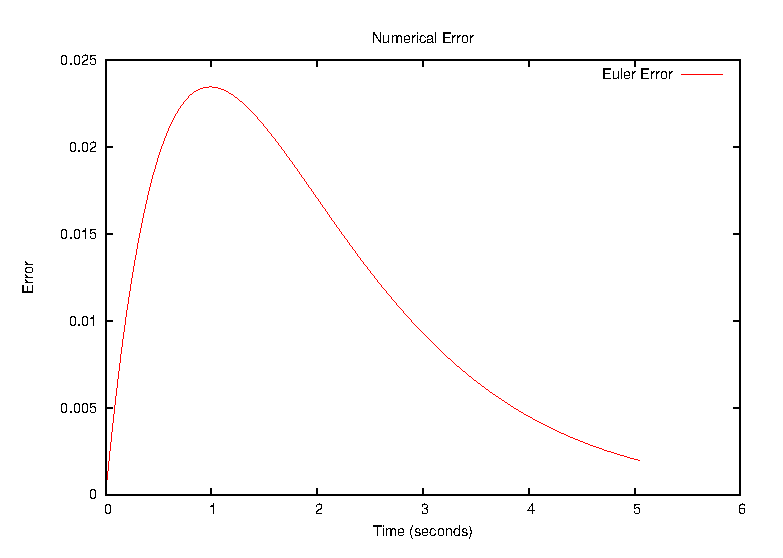
\epsfig{file=data/part1/figures/eulerError,width=14cm,height=5.5cm}
\end{center}
\caption{\label{pict3}Error of Euler Method; A=2,I=0}
\end{figure}
 
\vfil\eject

Below you can see the plot of the numerical simuation using RK4. The input current, $I$, was turned on at $t=0$ and on at $t=5$. The Potential in the Leaky Integrator model naturally approaches an equilibrium value $\frac{I}{A}$, and changing $I$ at this time causes this equilibrium value to change

\begin{figure}[h!]
\begin{center}
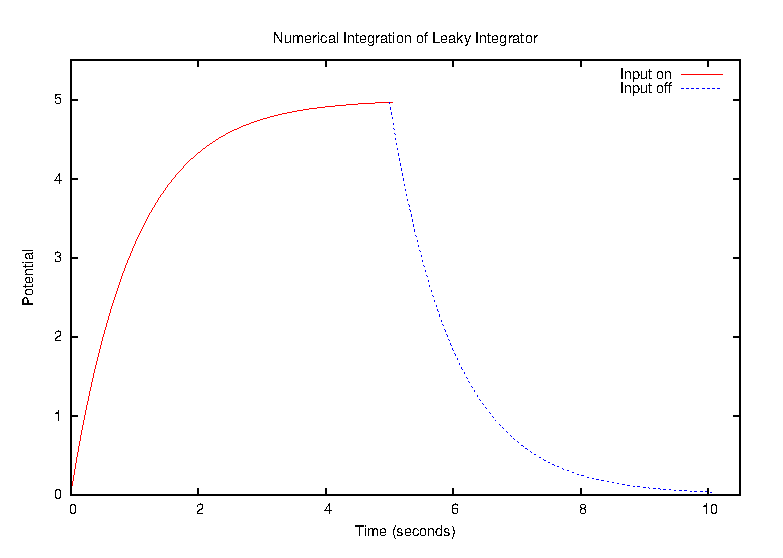
\epsfig{file=data/part1/figures/rk1,width=14cm,height=7cm}
\end{center}
\caption{\label{pict1}Numerical Simulation 1; A=1, I=5(on),0(off)}
\end{figure}

\begin{figure}[h!]
\begin{center}
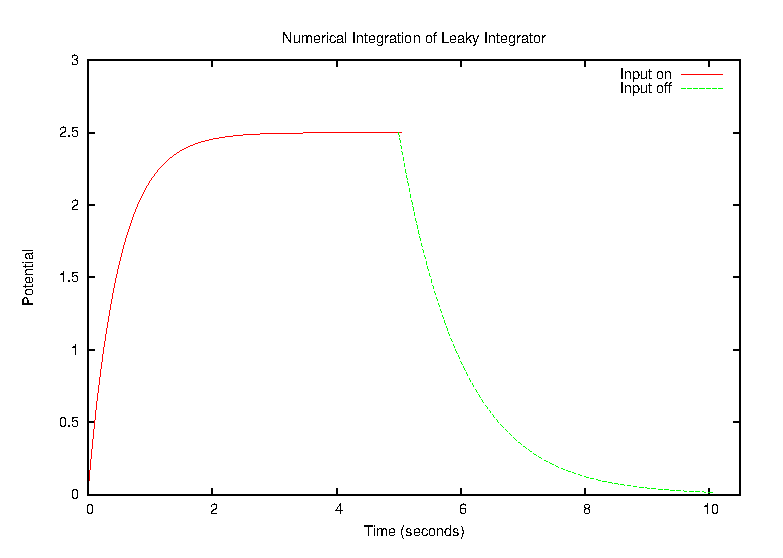
\epsfig{file=data/part1/figures/rk2,width=14cm,height=7cm}
\end{center}
\caption{\label{pict2}Numerical Simulation 2; A=2, I=5(on),0(off)}
\end{figure}

\vfil\eject

{\bf Discussion}
\bigskip

I chose to include the results to the RK4 simulation because I've been lead to believe they are more accurate. If the grader would like to see the Euler results, it is no trouble for me to submit them. As previously discussed the Euler method exhibited a small degree of error when compared to the Analytic solution, though this error rapidly falls to zero as the solution converges. 

\vspace{2mm}

It is worthwhile noting that the numerical error seems to peak at t=1 before falling off; looking at the equation for the Leaky Integrator, we see that it uses an exponential term in its time evolution. In general this term vanishes as $t$ grows large, but for values of $t<1$, my hypothesis is that the exponential term will vanish at a slower rate. This will cause the error to build up until that term starts to approach zero at an increased rate, thus bringing the system to equilibrium. 

\vspace{2mm}

These numerical solutions are a necessity as the differential equations we deal with become less tractable, but there is an obvious tradeoff between computation time and accuracy. It seems to me that the best integration method was Rotter-Deissmann; it performed as many operations as Euler, but yielded results as accurate as RK4. 

\vfil\eject

\bigskip
{\bf Part 2 : Leaky Integrate and Fire}
\vspace{2mm}
{\bf Introduction}
\bigskip

The second part of the assignment asks us to simulate the Leaky Integrator with a modification that causes it to spike at certain threshold values. What this means is that when the solution to 

\begin{equation}
\frac{dx}{dt}+Ax=I
\end{equation}

cross some threshold value, $vThresh$, the potential value will automatically spike to some arbitrarily high value, called $vSpike$. In order to do this, we need to hard-code an update and reset condition in our original leaky integrator that checks our solution against this threshold and, if we've crossed it, generate a spike. Once the spike is generated, we reset the potential so a value called $vReset$. 

\vspace{2mm}

It should be noted that this is not a natural feature of the Leaky Integrator model. These spikes must be hard coded using 'if' statements, and are set to fire once the potential crosses our threshold. The simulation was run using two threshold values: $vThresh = 1,2$. The simulation runs for $10$ seconds, during which the input current $I$ is on for $1<=t<=6$ and set to a value of $3$. 

\vspace{2mm}

I decided to keep my Rotter-Deissmann and Runge Kutta code from the last assignment, so I ran the simulation using those two methods along with Euler. I must admit that I struggled for some time with an analyitic simulation of the firing, only to discover that it cannot be done using the solution I found to the leaky integrator. The numerical methods work because they allow the system to adapt no matter where it is. The analytic solution is aware of what time it's at in the simulation, so when I tried to simulate spiking it had already converged toward equilibrium; $\frac{I}{A}$ is greater than any value of $vThresh$, so I got five seconds of radical spikes. 

\vspace{2mm}

I chose a spike value $vSpike = 50$, and a reset value $vReset = -1$. 

\vspace{2mm}

I've attached the source code for this model to this submission; all changes required for this model can be found in the individual simulation methods, i.e solveRK, solveE, solveRD. 

\vfil\eject

{\bf Results}
\bigskip

Below you can see the plots of the Leaky Integrate and Fire neuron using two different spike threshold values. 

\begin{figure}[h!]
\begin{center}
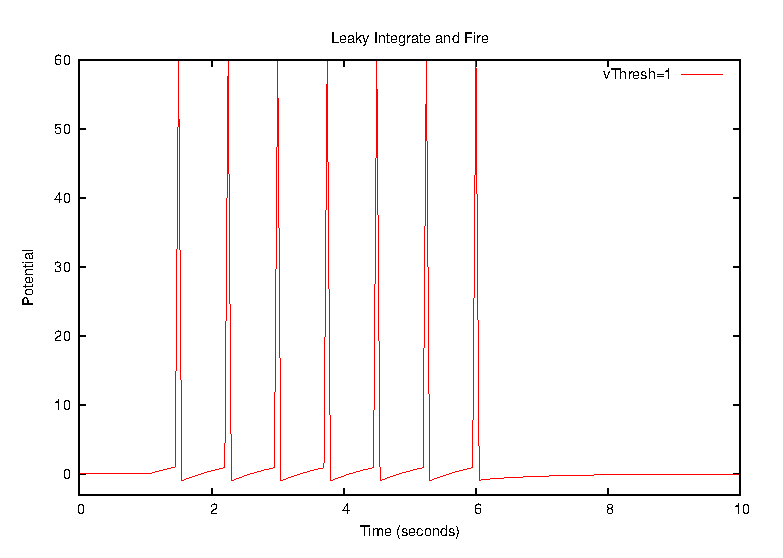
\epsfig{file=data/part2/figures/Vt1,width=14cm,height=7cm}
\end{center}
\caption{\label{pict4}Numerical Simulation 1; A=1, I=3(on),0(off)}
\end{figure}

\begin{figure}[h!]
\begin{center}
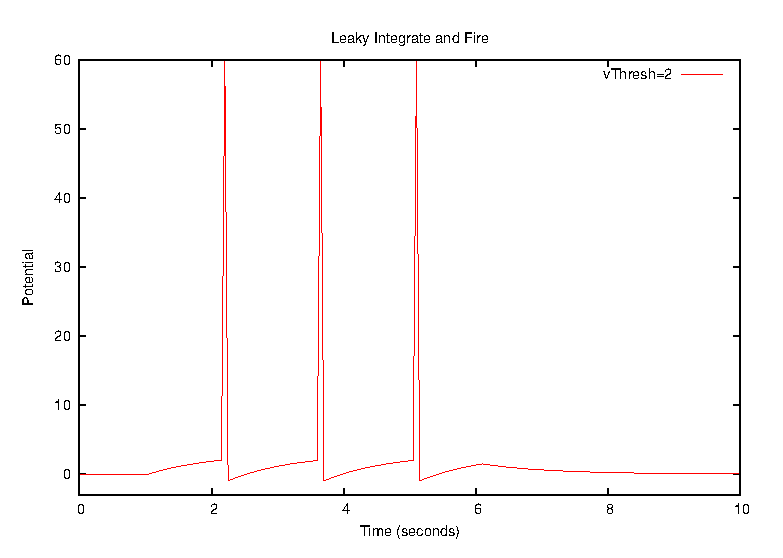
\epsfig{file=data/part2/figures/Vt2,width=14cm,height=7cm}
\end{center}
\caption{\label{pict5}Numerical Simulation 2; A=1, I=3(on),0(off)}
\end{figure}

\vfil\eject

The results for this simulation produced a nice series of spikes. The plots will be on the next page. The spiking rate was calculated for each simulation, though I did have some confusion as to how that should be measured. 

\vspace{2mm}

The first spike produced when $vThresh=1$ occured at $t=1.5$, and the last spike was at $t=6$. A total of seven spikes were observed, so the spike rate should be 

\begin{equation}
\frac{7}{6-1.5} = 1.56 \frac{spikes}{second}
\end{equation}

However, spikes were observed at the following times:

\begin{equation}
[ 1.5, 2.25, 3, 3.75, 4.5, 5.25, 6 ]
\end{equation}

It is plain to see that there was a spike every $0.75$ seconds, meaning the spike rate should be $1.33 \frac{spikes}{second}$. 

\vspace{2mm}

When $vThresh = 2$, the first spike rate equation is 

\begin{equation}
\frac{3}{5.1-2.2} = 1.03 \frac{spikes}{second}
\end{equation}

However, spikes were observed at the following times:

\begin{equation}
[ 2.2, 3.65, 5.1 ]
\end{equation}

Which puts a spike every $1.45$ seconds, making the spiking rate $0.69 \frac{spikes}{second}$. The ratio of these spiking rates is either $1:0.66$ if you follow the instructions, or $1:0.52$ if you look at the data, though either way it seems as though the ratio of rates is nealy the reciprocal of the ratio of threshold values. 

\vspace{2mm}

Given that the input current is only turned on at $t=1$, the first simulation saw its first spike $0.5$ seconds into the ``on'' portion. The second simulation saw its first spike $1.2$ seconds into the ``on'' portion, and the ratio of these two numbers is $1:2.4$. 

\vspace{2mm}

A change in A from 1 to 2 means doubling the decay rate of the system and halving its equilibrium value. An equilibrium value of $\frac{I}{A} = \frac{3}{2}$ means that for $vThresh = 1$ we would see more spikes, but for $vThresh = 2$ we would not see any spikes. This is because an increase in A causes the system to converge more quickly, but also means it converges to a value too low to cross the second threshold. 

\end{document}
